\section{Abelian varieties: CM points and propagation}\label{sec:abelian}

\subsection{The statement \texorpdfstring{\st{CM}}{(CM)}}\label{ssec:cmclaim}
Let $A$ be an abelian variety of CM type. Its Hodge group is a torus, and
after extending scalars to a Galois CM field $E$ that splits it, $H^{1}(A)$
is a sum of lines indexed by embeddings, each of type $(1,0)$ or $(0,1)$.
Deligne and Andr\'e showed that every Hodge class on $A$ is a sum of
pull-backs, along homomorphisms $A\to A_{\Delta}$, of Weil classes on
abelian varieties $A_{\Delta}$ of split Weil type \cite[Theorem~1]{Mil20}.
So \st{CM} is equivalent to the algebraicity of these split Weil classes, and
it is open in the refereed literature.

The preprint \cite{OAI26} claims \st{CM} \cite[Theorem~1.1]{OAI26}. Its proof
has four steps. (1) The theorem is reduced \cite[Proposition~2.6]{OAI26} to
the algebraicity of a line of type $(2,2)$ on a product of four CM abelian
varieties $B(v_{1}),\dots,B(v_{4})$, attached to odd sign functions
$v_{i}\colon\operatorname{Gal}(E/\QQ)\to\{\pm1\}$ with $v_{1}+v_{2}=v_{3}+v_{4}$
\cite[Theorem~2.5]{OAI26}. (2) That line is shown to be algebraic as soon as
four degree-one classes on a surface, coming from the four CM Hodge
structures, have a nonzero mixed period \cite[Proposition~3.1]{OAI26}. (3)
Such a period is produced by theta forms on compact quotients of the complex
two-ball \cite[\S4]{OAI26}. (4) The theta classes are shown to come from the
prescribed CM Hodge structures, through Hecke operators and a Frobenius
relation on the reductions of the ball quotients \cite[Theorem~5.1 and
Corollary~6.7]{OAI26}.

We have checked the combinatorial part of step (1): its core is
\Cref{lem:switch} below, and its contraction formula
\cite[(2.6)]{OAI26} carries the sign $(-1)^{p(p-1)/2}$, which we recompute in
\Cref{app:checks}. We have not checked steps (2) to (4), and the claim rests
on step (4). Accordingly, every result of this paper that uses \st{CM}
states it as a hypothesis.

\begin{lemma}[Two-row switches]\label{lem:switch}
Let $G$ be a finite set with a fixed-point-free involution $c$, let
$s=|G|/2$, and call $v\colon G\to\{\pm1\}$ \emph{odd} if $v(cg)=-v(g)$. Let
$x=(x_{1},\dots,x_{p})$ and $y=(y_{1},\dots,y_{p})$ be lists of odd functions
with $\sum_{i}x_{i}=\sum_{i}y_{i}$. Then there is a chain of lists of odd
functions $x=x^{(0)},x^{(1)},\dots,x^{(N)}=y$ with $N\le s\lfloor
p/2\rfloor$, in which $x^{(k+1)}$ differs from $x^{(k)}$ in exactly two
entries $i\ne j$, and $x^{(k+1)}_{i}+x^{(k+1)}_{j}=x^{(k)}_{i}+x^{(k)}_{j}$.
\end{lemma}

\begin{proof}
Choose a set $T$ of representatives of the orbits of $c$; an odd function is
determined by its values on $T$. Treat the elements $\tau\in T$ one at a
time. Let $P_{\tau}$ be the set of indices $i$ with $x_{i}(\tau)=1$ and
$y_{i}(\tau)=-1$, and $N_{\tau}$ the set with $x_{i}(\tau)=-1$ and
$y_{i}(\tau)=1$. Then $\sum_{i}x_{i}(\tau)-\sum_{i}y_{i}(\tau)=2|P_{\tau}|-
2|N_{\tau}|$, so $|P_{\tau}|=|N_{\tau}|\le\lfloor p/2\rfloor$. Pair the two
sets, and for each pair $(i,j)$ exchange the values of the $i$-th and $j$-th
functions at $\tau$ and at $c\tau$. Each exchange keeps the functions odd,
changes exactly the entries $i$ and $j$, and keeps their sum, since it only
swaps two values at each of two points. After the pairs for $\tau$ are
exchanged, the list agrees with $y$ at $\tau$ and $c\tau$, and the later
steps do not change these values.
\end{proof}

In \cite{OAI26} the lists come from the types of the factors of a Hodge
monomial, a two-row switch is exactly a relation $v_{1}+v_{2}=v_{3}+v_{4}$,
and the algebraic tensors of consecutive switches are composed by
contracting the middle factors against an ample class
\cite[(2.6)]{OAI26}.\footnote{The contraction multiplies by
$(-1)^{p(p-1)/2}\prod_{i}q_{i}$, where the sign comes from regrouping
$\beta_{1}\cdots\beta_{p}\gamma_{1}\cdots\gamma_{p}$ as
$\beta_{1}\gamma_{1}\cdots\beta_{p}\gamma_{p}$ for classes of degree one, and
$q_{i}=\int_{B(b_{i})}\beta_{i}\wedge\gamma_{i}\wedge\ell_{i}^{s-1}$ is
nonzero by the Hodge--Riemann relations, because $\gamma_{i}$ is a nonzero
multiple of $\bar\beta_{i}$.} Nothing in this combinatorial part depends on
the geometry of steps (2) to (4).

\subsection{Propagation from CM points}

\begin{lemma}[CM points are dense]\label{lem:cmdense}
Let $G$ be a connected reductive group over $\QQ$, let
$u_{0}\colon\U(1)\to G_{\RR}$ be a homomorphism, and let $\cD$ be its orbit
under conjugation by $G(\RR)^{+}$. The points $u\in\cD$ with
$u(\U(1))\subseteq T_{\RR}$ for a maximal torus $T$ of $G$ defined over
$\QQ$ are dense in $\cD$.
\end{lemma}

\begin{proof}
Let $u_{1}\in\cD$ and let $W$ be a neighbourhood of $u_{1}$. A maximal torus
$T_{1}$ of $G_{\RR}$ contains the torus $u_{1}(\U(1))$; let
$\mathfrak{t}_{1}$ be its Lie algebra and $Y_{1}\in\mathfrak{t}_{1}$ a regular
element. The map $\phi\colon G(\RR)^{+}\times\mathfrak{t}_{1}\to
\mathfrak{g}_{\RR}$, $(g,Y)\mapsto\operatorname{Ad}(g)Y$, has differential
$(Z,Y')\mapsto[Z,Y_{1}]+Y'$ at $(1,Y_{1})$, which is onto because
$\mathfrak{g}_{\RR}=\mathfrak{t}_{1}\oplus[\mathfrak{g}_{\RR},Y_{1}]$ for a
regular semisimple $Y_{1}$. So for small neighbourhoods $N_{1}$ of $1$, with
$N_{1}u_{1}N_{1}^{-1}\subseteq W$, and $N_{2}$ of $Y_{1}$ consisting of
regular elements, $\phi(N_{1}\times N_{2})$ contains a nonempty open set,
and hence a rational element $Y=\operatorname{Ad}(g)Y'$ with $g\in N_{1}$,
$Y'\in N_{2}$. The identity component $T$ of the centralizer of $Y$ is a
maximal torus defined over $\QQ$, and $T_{\RR}=gT_{1}g^{-1}$. Then
$u=gu_{1}g^{-1}\in W$ and $u(\U(1))\subseteq T_{\RR}$.
\end{proof}

\begin{proposition}[A CM member through every Hodge class]\label{prop:cmfamily}
Let $A_{0}$ be an abelian variety and $\gamma$ a Hodge class of degree $2p$
on $A_{0}$. There are a polarized abelian scheme $\pi\colon\cA\to S$ over a
smooth connected quasi-projective variety, a global section $\xi$ of
$R^{2p}\pi_{*}\QQ$, and points $s_{0},c\in S$, such that
$\cA_{s_{0}}\cong A_{0}$ with $\xi_{s_{0}}=\gamma$, $\xi_{s}$ is a Hodge class
for every $s$, and $\cA_{c}$ is of CM type.
\end{proposition}

\begin{proof}
Replacing $\gamma$ by a multiple, we may assume it integral. Fix a
polarization of $A_{0}$ with form $\psi$ on $V=H_{1}(A_{0},\QQ)$, and a level
$N\ge3$. The complex structures $J$ on $V_{\RR}$ that are compatible with
$\psi$ and positive for it form the Siegel space $\mathcal{H}$, and its
quotient $\mathcal{S}$ by the principal congruence subgroup of level $N$ in
$\operatorname{Sp}(H_{1}(A_{0},\ZZ),\psi)$ is a smooth quasi-projective
variety with a universal polarized abelian scheme $f\colon\cA_{g}\to
\mathcal{S}$ \cite[Chapter~7]{MFK94}. Let $\mathbb{V}=R^{2p}f_{*}\ZZ$. By
the theorem of Cattani, Deligne and Kaplan \cite[Theorem~1.1]{CDK95}, the
set of pairs $(a,v)$, with $a\in\mathcal{S}$ and $v\in\mathbb{V}_{a}$ an
integral Hodge class with the same self-intersection as $\gamma$, is a closed
algebraic subvariety of the total space of the vector bundle
$\mathbb{V}\otimes\cO_{\mathcal{S}}$, finite over $\mathcal{S}$; let
$\mathcal{C}$ be its connected component through the point $(a_{0},\gamma)$
given by $A_{0}$ and a lift $J_{0}\in\mathcal{H}$.

Let $G\subseteq\operatorname{Sp}(V,\psi)$ be the Hodge group of $A_{0}$, the
smallest algebraic subgroup over $\QQ$ whose real points contain the image
of the homomorphism $u_{0}\colon\U(1)\to\operatorname{GL}(V_{\RR})$,
$e^{i\theta}\mapsto\cos\theta+J_{0}\sin\theta$. It is connected and
reductive, and it fixes every Hodge class of $A_{0}$, in particular $\gamma$
\cite[\S3]{Del82}. For $g\in G(\RR)^{+}$ the structure $J=gJ_{0}g^{-1}$ lies
in $\mathcal{H}$, and the Hodge group of $A_{J}$ is contained in $G$, so
$\gamma$ is a Hodge class on $A_{J}$. The orbit $\cD=\{gJ_{0}g^{-1}\}$ is
connected, so its image $J\mapsto(a_{J},\gamma)$ lies in $\mathcal{C}$. By
\Cref{lem:cmdense} there are $J_{k}\in\cD$ converging to $J_{0}$ such that
$u_{J_{k}}(\U(1))$ lies in a torus defined over $\QQ$; the Hodge group of
$A_{J_{k}}$ is then commutative, and $A_{J_{k}}$ is of CM
type.\footnote{The torus $T$ lies in a maximal torus $T'$ of
$\operatorname{GL}(V)$ over $\QQ$, the units of a commutative semisimple
subalgebra $L\subseteq\End(V)$ of dimension $2g$. Since $L$ commutes with
$T'\supseteq\Hg(A_{J_{k}})$, it lies in the commutant of the Hodge group,
which is $\End(A_{J_{k}})\otimes\QQ$.} One of the finitely many irreducible
components of $\mathcal{C}$, say $\mathcal{C}_{0}$, contains infinitely many
of the points $(a_{J_{k}},\gamma)$, and, being closed, also their limit
$(a_{0},\gamma)$.

Let $S\to\mathcal{C}_{0}$ be a resolution of singularities \cite{Hir64}, so
that $S$ is smooth, connected and quasi-projective, and let $\cA\to S$ be the
pull-back of $\cA_{g}$. The total space of a local system is a covering space
of the base, so $(a,v)\mapsto v$ is a flat section on $\mathcal{C}_{0}$, and
its pull-back is a global section $\xi$ of $R^{2p}\pi_{*}\ZZ$ that is a Hodge
class at every point. Take $s_{0}$ over $(a_{0},\gamma)$ and $c$ over some
$(a_{J_{k}},\gamma)$.
\end{proof}

\begin{proposition}\label{prop:cmip}
\st{F2} holds if and only if both \st{CM} and \st{IP} hold.
\end{proposition}

\begin{proof}
\st{F2} contains \st{CM}, and it implies \st{IP}: if $\xi_{c}$ is algebraic,
then every $\xi_{s}$ is a Hodge class by \Cref{lem:fixed}, hence algebraic.
Conversely, let $\gamma$ be a Hodge class on an abelian variety $A_{0}$, and
take $\pi$, $\xi$, $s_{0}$ and $c$ from \Cref{prop:cmfamily}. Then $\xi_{c}$
is a Hodge class on an abelian variety of CM type, so it is algebraic by
\st{CM}, and by \st{IP} the class $\gamma=\xi_{s_{0}}$ is algebraic.
\end{proof}

The proposition separates the two inputs of the argument of Deligne and
Andr\'e as Milne records it \cite[\S5]{Mil20}: the classes at CM points, and
their transport along families. The variational conjecture \st{V} supplies
both at once \cite[Theorem~3 and Remark~2]{Mil20}, because the split Weil
classes are algebraic at a suitable member of each family
\cite[4.8]{Del82}. \st{IP} supplies only the transport, and it does so only
from CM members.

\subsection{Proof of \texorpdfstring{\Cref{thm:A}}{Theorem A}}\label{ssec:proofA}
By \Cref{lem:hcimplies}, (i) implies each of (ii)--(vi). If \st{F2} holds,
every $\gamma$ in the definition of $\Ab^{p}(X)$ is algebraic, so
$\Ab^{p}(X)=\Alg^{p}(X)$, and \st{F3$'$} becomes \HC; so (ii) implies (i).
\st{L} implies \st{F2} by the theorem of Abdulali and Andr\'e
\cite[Theorem~4]{Mil20}\footnote{Milne's hypothesis is the Lefschetz
standard conjecture in the form that $L^{d-2i}$ maps the algebraic classes
of degree $2i$ onto those of degree $2d-2i$. It follows from \st{L}, since
the inverse of $L^{d-2i}$ is then induced by an algebraic cycle and maps
algebraic classes to algebraic classes.}, \st{V} implies \st{F2}
\cite[Theorem~3 and Remark~2]{Mil20}, and \st{CM} with \st{IP} implies
\st{F2} by \Cref{prop:cmip}; so (iii), (iv) and (v) imply (ii). Finally (vi)
implies (i) by \Cref{prop:LM}. \qed

\subsection{Weil families and degrees at CM points}\label{ssec:weilfamilies}

Let $K$ be an imaginary quadratic field and $n\ge1$. An abelian variety $A$
of dimension $2n$ with an action of $K$ is \emph{of Weil type} if both
embeddings of $K$ occur with multiplicity $n$ on $H^{1,0}(A)$. Then the
\emph{Weil plane} $W(A)=\bigwedge^{2n}_{K}H^{1}(A,\QQ)\subseteq
H^{2n}(A,\QQ)$ is a $\QQ$-plane of Hodge classes \cite{Wei77},
\cite[\S4]{Del82}. For a polarization whose Rosati involution induces
complex conjugation on $K$, the Riemann form is
$\operatorname{Tr}_{K/\QQ}(f H)$ for a $K$-hermitian form $H$ of signature
$(n,n)$, and $A$ is \emph{of split Weil type} if $H$ has a totally isotropic
$K$-subspace of dimension $n$ \cite[\S2.1]{Mil20}.

Fix such data and a level $N\ge3$. The abelian varieties of split Weil type
for $(K,n)$ with this hermitian form and level structure are parametrized by
a smooth connected quasi-projective variety $S$, a quotient $\Gamma\backslash
\cD$ of the hermitian symmetric domain $\cD$ of $\SU(n,n)$, of dimension
$n^{2}$, by a neat arithmetic subgroup $\Gamma$ of the unitary group; it is a
connected Shimura variety of PEL type and carries a polarized abelian scheme
$\pi\colon\cA\to S$ with an action of $\cO_{K}$
\cite{Wei77,vG94}.\footnote{The unitary group acts on the Weil plane through
the determinant. For $\gamma\in\Gamma$ the determinant is a unit of $\cO_{K}$
of norm one, hence a root of unity, and it is $1$ because $\Gamma$ is neat.
So the Weil planes of the members form a trivial local system on $S$, and
every Weil class on one member extends to a global section.} The special
points of $S$ are the members of CM type. Fix a nonzero global section $\xi$
of the Weil planes. An element $\alpha\in\cO_{K}$ acts on $\cA_{s}$, and its
pull-back multiplies the $K$-line $W(\cA_{s})$ by $\alpha^{2n}$. Choose
$\alpha$ with $\alpha^{2n}\notin\QQ$.\footnote{The $\alpha\in K\otimes\RR=\CC$
with $\alpha^{2n}$ real lie on $2n$ lines through $0$, and the lattice
$\cO_{K}$ is not contained in finitely many lines.} Then $\alpha^{*}$ moves
any nonzero class of $W(\cA_{s})$ to a class that spans $W(\cA_{s})$ with it,
and pull-back by an endomorphism preserves algebraic classes; so
$W(\cA_{s})$ consists of algebraic classes exactly when $\xi_{s}$ is
algebraic.

\begin{definition}\label{def:sigmad}
Let $\Sigma\subseteq S$ be the set of $s$ at which $\xi_{s}$ is algebraic.
For $d\ge1$ let $\Sigma_{d}$ be the set of $s$ for which there are effective
algebraic cycles $Z^{+},Z^{-}$ of codimension $n$ on $\cA_{s}$, each of
degree at most $d$ for the polarization, and an integer $1\le e\le d$, with
$e\,\xi_{s}=\cl(Z^{+})-\cl(Z^{-})$.
\end{definition}

\begin{lemma}\label{lem:sigmaclosed}
Each $\Sigma_{d}$ is Zariski closed in $S$, $\Sigma_{d}\subseteq\Sigma_{d+1}$,
and $\Sigma=\bigcup_{d}\Sigma_{d}$.
\end{lemma}

\begin{proof}
The last two assertions are clear. Effective cycles of codimension $n$ and
degree at most $d$ in the fibres of $\pi$ are parametrized by finitely many
relative Chow varieties $\mathcal{C}_{i}\to S$, which are projective over $S$
\cite[Chapter~I, \S\S3--4]{Kol96}. On a connected component of
$\mathcal{C}_{i}\times_{S}\mathcal{C}_{j}$ the class $\cl(Z^{+})-\cl(Z^{-})$
of the fibre is a flat section of the pulled-back local system, and so is
$e\,\xi$. Two flat sections over a connected base that agree at one point
agree everywhere, so the set where they agree is a union of connected
components. Its image in $S$ is closed, because the projection is proper.
$\Sigma_{d}$ is the union of finitely many such images.
\end{proof}

\begin{proof}[Proof of \Cref{thm:D}]
The first sentence is \Cref{lem:sigmaclosed}. (ii) implies (i) trivially. If
(i) holds, $S^{\mathrm{an}}$ is the countable union of the closed sets
$\Sigma_{d}$, so by the Baire category theorem one of them has an interior
point; a Zariski closed subset of the irreducible variety $S$ with an
interior point is $S$, which gives (ii). If (ii) holds, the CM points in
$\Sigma_{d}=S$ are dense in $S^{\mathrm{an}}$ by \Cref{lem:cmdense}, so they
lie in no finite union of proper closed subvarieties, which gives (iii).
Assume (iii), and let $Z$ be the Zariski closure of the set of CM points in
$\Sigma_{d}$; it lies in $\Sigma_{d}$. Every irreducible component of $Z$
contains a Zariski dense set of special points, so it is a special
subvariety, by the Andr\'e--Oort conjecture, which is a theorem
\cite{PST21}. By (iii) one of these components is not proper, so
$S\subseteq Z\subseteq\Sigma_{d}$, which is (ii). Finally, at a CM point
$\xi_{s}$ is a Hodge class on an abelian variety of CM type, so under
\st{CM} it is algebraic.
\end{proof}

\begin{figure}[t]
\centering
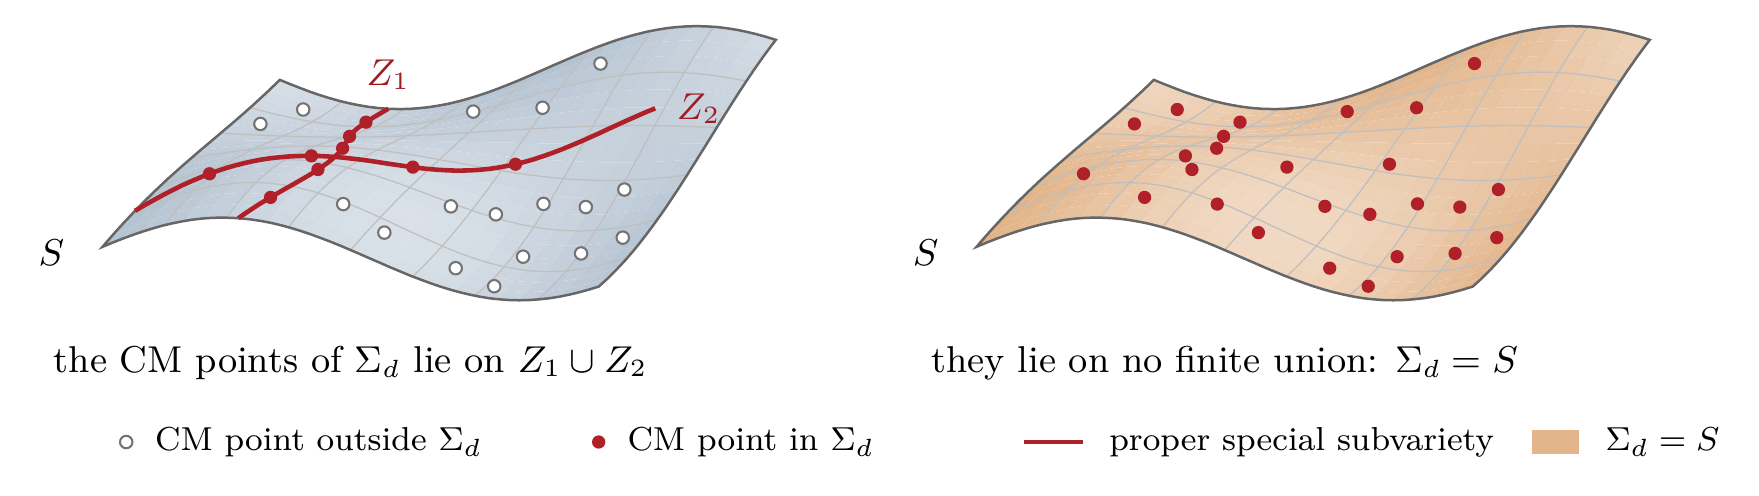
\includegraphics[width=\textwidth]{figures/fig_locus}
\caption{The criterion of \Cref{thm:D}, drawn schematically ($S$ has
dimension $n^{2}$). CM points are dense in $S$. On the left the CM points
of $\Sigma_{d}$ lie on two proper special subvarieties $Z_{1}$ and $Z_{2}$,
and condition (iii) fails for this $d$. On the right they lie on no finite
union of proper special subvarieties; by the Andr\'e--Oort theorem their
Zariski closure is then $S$, and $\Sigma_{d}=S$.}
\label{fig:locus}
\end{figure}

\begin{remark}\label{rem:degrees}
Without any hypothesis $\Sigma$ is dense. It contains the members
$K$-isogenous to $E^{n}\times\bar E^{n}$, which is of split Weil type and
whose Weil classes are polynomials in divisor classes (\Cref{lem:EEbar});
and with every point it contains its Hecke orbit, which is dense. Algebraic representatives move
along isogenies by push-forward and pull-back, and their degree grows with
the degree of the isogeny. \st{CM} adds every CM point, but it gives no bound
on the degrees, and by \Cref{thm:D} a bound on a set of CM points that is
not trapped in finitely many proper Shimura subvarieties is exactly what
remains. Neither \cite{OAI26} nor any other source we know gives such a
bound.
\end{remark}
